% ------------------------------------------------------------------------
%%%%% Start of preamble %%%%%
% ------------------------------------------------------------------------

%%%%---------What kind of document  and what size--------------------------------------
\documentclass[12pt]{article}

%%%MY: Other possible document: article, report, amsart, thesis, book,etc.


%%%%---------Packages to load which give you useful commands---------------------------------
\usepackage{graphicx} %to include pictures and figures
\usepackage{amssymb, amsmath, amsthm} %to include standard Americam Mathematical Society math symbols and fonts
\usepackage{fontenc} %to be able to inlude more font
\usepackage{amscd,latexsym,amsfonts,amstext,amsbsy} %more AMS fonts and options
\usepackage{euscript} %for european script
\usepackage{enumerate} %for automatic enumeration of equations, items, etc.
\usepackage{color}  %to change the color of a text.
\usepackage{physics}
\usepackage[latin1]{inputenc}
\usepackage{tikz}
\usepackage{mathrsfs}
\usetikzlibrary{shapes,arrows}


%%%%---------Sets the margins--------------------------------------------------------------
%As example, the margins are manually chosen below.  You can change the margins if needed.
%%%In particular: Use default margins first (just insert % the the start of each of
%the lines below for LaTex to disregard the options, ---------------------

\textwidth = 16 cm
\textheight = 24 cm
\oddsidemargin = 0.0 cm
\evensidemargin = 0.0 cm
\topmargin = -2 cm
%\headheight = 0.0 in
%\headsep = 0.0 in
\parskip = 0.2in
\parindent = 0.0in

%%%%------------MY: sets up doublespacing: use 2  inside the {} below---------------------------------
%This allows me to include feedback between the lines.
%For singlespace  just use % to disregard the command or use 1 instead.
%\renewcommand{\baselinestretch}{2}


%%%---------------MY: New theorem type environments-------------------------------
 \newtheorem{theorem}{Theorem}
  \newtheorem{problem}[theorem]{Problem}
   \newtheorem{exercise}[theorem]{Exercise}
 \newtheorem{corollary}[theorem]{Corollary}
 \newtheorem{lemma}[theorem]{Lemma}
 \newtheorem{proposition}[theorem]{Proposition}
 \newtheorem{proporties}[theorem]{Proporties}
 \newtheorem{definition}[theorem]{Definition}
  \newtheorem{definitions}[theorem]{Definitions}
  \newtheorem{example}[theorem]{Example}
 \newtheorem{remark}[theorem]{Remark}
 


\begin{document}
%%%%%%This declares that your document starts here
\textbf{Heroin Model} \\
Tricia Phillips \\
\today \\

\textbf{Background} \\ \\**Talk about fetanyl ("America's")
The misuse of opioids, a drug class including prescription pain relievers and the illegal drug heroin, is rampant in today's society. The opioid crisis was declared a public health emergency in October 2017 by the United States Department of Health and Human Sciences [15]. In 2016, there were 11.8 million opioid misusers 12 years of age or older with 948,000 of these being heroin users [10]. In addition, there was an estimated 13,219 heroin deaths in 2016, a more than six-fold increase from the year 2002 [7]. 

Prescription pain relievers are misused for a variety of reasons with the most prominent being to relieve physical pain, to feel good or get high and to relax or relieve tension [10]. Individuals that misuse prescription opioids mostly obtain them from friends/relatives or from a healthcare provider, with misuse defined as taking the prescription at a higher dose or more frequently than prescribed, or taking someone else's medication [10]. 

To address this apparent problem in today's society, we have formulated a population level model to investigate the dynamics among individuals taking prescription opioids, addicted to opioids, using heroin and recovering from addiction. We aim to find ways to reduce opioid addiction and heroin use and plan to investigate how to optimally treat pain while reducing the risk of addiction lower than it's current state. This model was motivated by a previous model focusing solely on opioid addicts through prescriptions or via the black market; the purpose of formulating a separate model is to be able to understand the more complicated dynamics that arise among opioid abuse and heroin use [1].  

\textbf{Model Formulation} \\ \\
Our model consists of five subgroups of the national population: 

1. Susceptibles ($S$): This portion of the population consists of individuals who are not taking prescription opioids of any kind, nor are using heroin. \\ \\
2. Prescription opioid users ($P$): This class of individuals consists of individuals who are prescribed opioids by a health care provider and take the opioids as recommended by their doctor, so they are not considered addicted. \\ \\
3. Opioid addicts ($A$): This group of individuals are addicted to opioids. Although the opioid class of drug includes heroin, here we will take opioids to mean non-heroin. In addition, opioid misuse, abuse and addiction will be used interchangeably throughout.  \\ \\
4. Heroin users ($H$): This class is composed of individuals who use heroin, which is implicitly understood to be addictive. \\ \\
5. Individuals in treatment/rehabilitation ($R$): This class consists of individuals undergoing treatment for their addiction to opioids and heroin. 

We denote the initial conditions as
$S(0)=S_{0}$, $P(0)=P_{0}$, $A(0)=A_{0}$, $H(0)=H_{0}$, and $R(0)=R_{0}$, and we assume all of these values are positive. From data, the initial values for each of the classes are the following proportions of the entire population: $S_{0}=0.6221$, $P_{0}=0.37$, $A_{0}=0.0062$, $H_{0}=0.0014$, and $R_{0}=0.0003$ [4],  **Will show that starting with positive initial conditions, will stay positive for all time. \\
%$\mu_{H} > \mu_{A}$ and $\theta_{3} > \theta_{1}, \theta_{2}$ 
\[\dv{S}{t} = -\alpha S - \beta (1- \xi) SA  -\beta \xi SP- \theta_{1} SH +\epsilon P +\delta R +\mu (P+R) + (\mu+\mu_{A})A + (\mu+\mu_{H}) H \quad (1)\] 
\[\dv{P}{t} = \alpha S - \epsilon P  - \gamma P - \theta_{2}PH- \mu P    \quad(2)\]
\[\dv{A}{t} = \gamma P + \sigma_{A} R +\beta (1- \xi) SA  +\beta \xi SP -\zeta A - \theta_{3}AH-(\mu + \mu_{A})A   \quad (3)\]
\[\dv{H}{t} = \theta_{1}SH+\theta_{2}PH+\theta_{3}AH + \sigma_{H}R-\nu H-(\mu+\mu_{H})H  \quad (4)\]
\[\dv{R}{t} = \zeta A +\nu H -\delta R -\sigma_{A}R-\sigma_{H}R -\mu R\quad(5)\]


The parameters involved in this model represent transition rates from one class to another; specifically: \\
$\alpha$: the rate at which people are prescribed opioids \\
$\beta$ : total probability of becoming addicted to opioids other than by prescription \\
$\beta(1-\xi)$: proportion of which the non-prescribed, susceptible population becomes addicted to opioids by black market drugs and other addicts \\
$\beta \xi$ : proportion of which the non-prescribed, susceptible population obtains extra prescription opioids and becomes addicted  \\
$\theta_1$: rate at which the non-prescribed, susceptible population becomes addicted to heroin by black market drugs and other addicts  \\
$\epsilon$: rate at which people come back to the susceptible class after being prescribed opioids and did not develop an addiction\\
$\delta$: rate at which people come back to the susceptible class after successfully finishing treatment \\
$\mu$: natural death rate \\
$\mu_A$: enhanced death rate for opioid addicts (overdose rate which results in death) \\
$\mu_H$: enhanced death rate for heroin addicts (overdose rate which results in death) \\
$\gamma$: rate at which prescribed opioid users become addicted \\
$\theta_2$: rate at which opioid prescribed user population becomes addicted to heroin \\
$\sigma_A$: rate at which people relapse from treatment into the opioid addicted class \\
$\zeta$: rate at which addicted opioid users enter treatment/rehabilitation \\
$\theta_3$: rate at which the opioid addicted population becomes addicted to heroin \\
$\sigma_H$: rate at which people relapse from treatment into the heroin addicted class \\
$\nu$: rate at which heroin users enter treatment/rehabilitation \\ 
This model can be represented by the following flow diagram: 

%\begin{center}
\begin{figure}
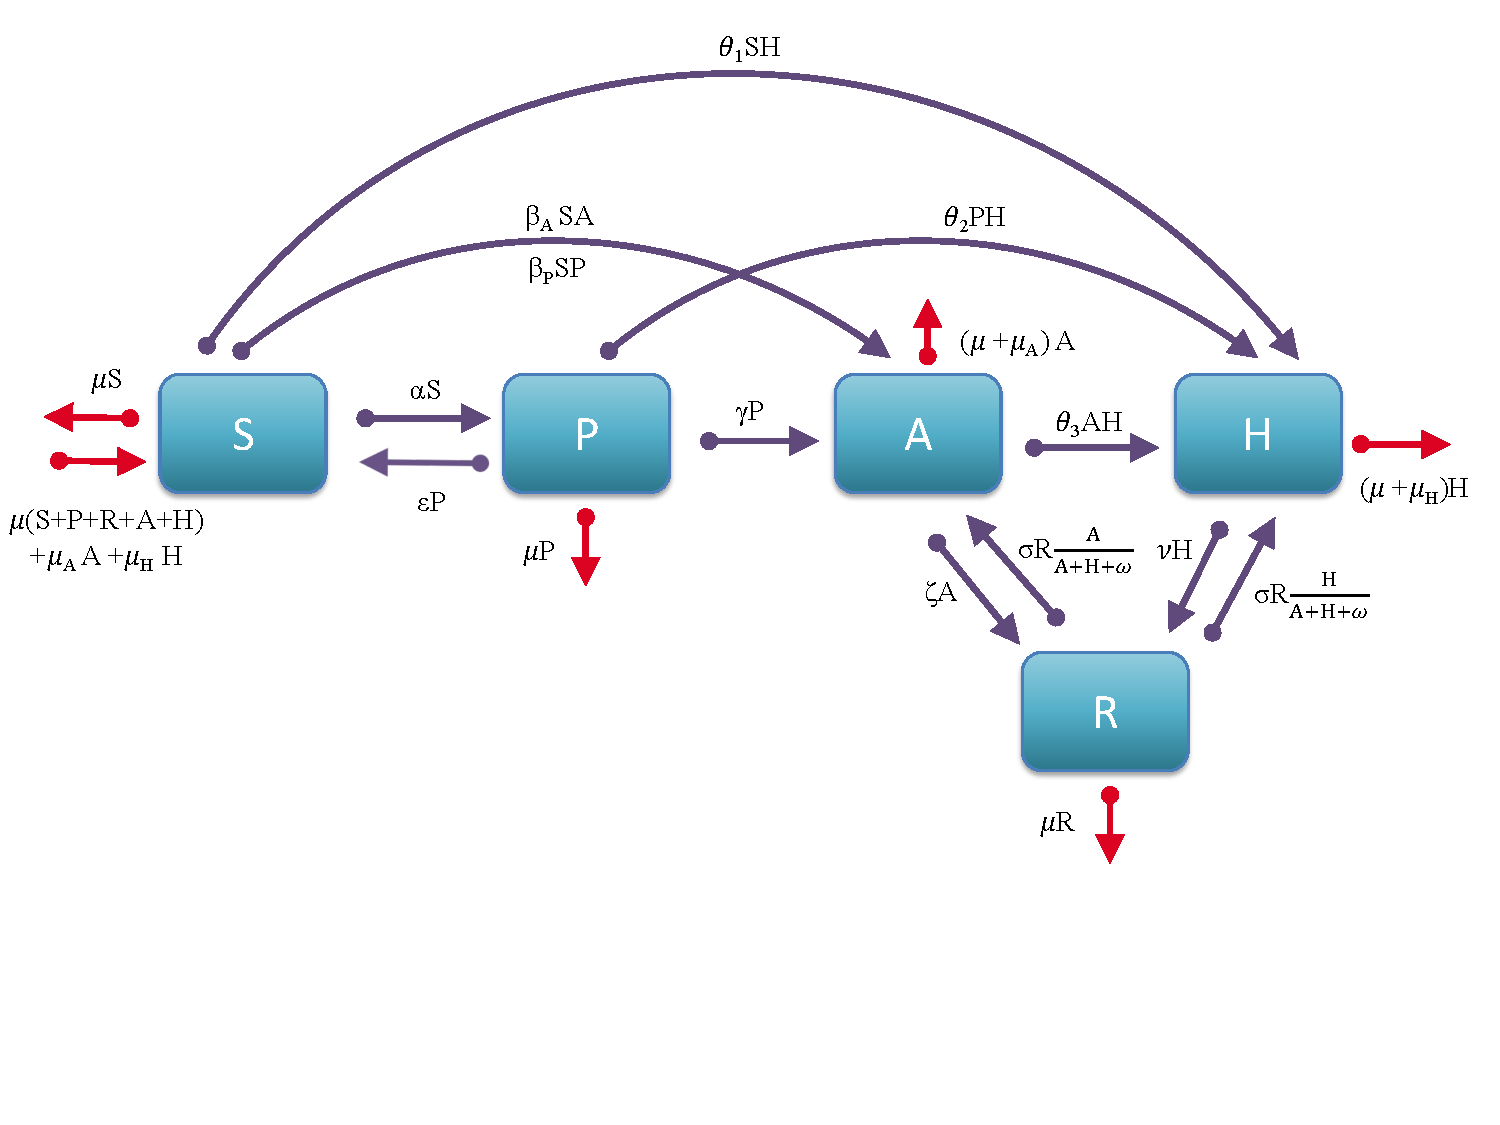
\includegraphics[scale=0.6]{heroin_schematic.pdf}
\end{figure}
%\end{center}
\textbf{Equilibrium Analysis} \\
**Find other equilibrium?? 
To find the addiction-free equilibrium, we set equations (1)-(5) equal to zero and require that $A=H=R=0$. We are left with the system: \\
\[0=-\alpha S^* -\beta \xi S^* P^* + \epsilon P^* +\mu P^* \quad\]
\[0=\alpha S^* - \epsilon P^* -\gamma P^* - \mu P^* \quad\]
\[0=\gamma P^* + \beta \xi S^* P^*   \quad\]



If $P=0$, then the only solution is $S^*=P^*=H^*=R^*=0$. Thus, will assume P $\neq 0. $ This forces $\gamma + \beta \xi S^* =0$ and since all of our parameters and variables are non-negative, then it must be $\gamma=0$ and either $\beta=0$ or $\xi=0$. Under the assumption that $\gamma=0=\xi$ to ensure the existence of our AFE and that $1=S+P+A+H+R$, we calculate the AFE to be \\

\[S^*=\frac{\epsilon + \mu}{\alpha + \epsilon +\mu}\quad\]
\[P^*=\frac{\alpha}{\alpha + \epsilon +\mu}\quad\]
\[A^*=0\quad\]
\[H^*=0\quad\]
\[R^*=0\quad\] \\

\textbf{Basic Reproduction Number, \textbf{$\mathscr{R}_0$}}

For the purposes of calculating $\mathscr{R}_0$, we will assume $\gamma =0$ and $\xi =0$ (thus, $\beta \neq 0$) in order to ensure the existence of the addiction-free equilibrium. This results in the infected compartment (3)-(5) reducing to:

\[\dv{A}{t} = \sigma_{A} R +\beta SA  -\zeta A - \theta_{3}AH-(\mu + \mu_{A})A   \quad\]
\[\dv{H}{t} = \theta_{1}SH+\theta_{2}PH+\theta_{3}AH + \sigma_{H}R-\nu H-(\mu+\mu_{H})H  \quad\]
\[\dv{R}{t} = \zeta A +\nu H -\delta R -\sigma_{A}R-\sigma_{H}R -\mu R\quad\]

Thus, under the assumption of A, H and R as the infected compartments and parameter restrictions stated above, the assumptions of the Next Generation Method are satisfied for matrices $\mathscr{F}$ and $\mathscr{V}$ shown below. Note that $\mathscr{F}_{i}$ represents the rate that secondary infections enter infected compartment $i$ and $\mathscr{V}_{i}$ represents the difference between the rate of transfer out of compartment $i$ and the rate of transfer into compartment $i$ by means different than a secondary infection. Using this method results in the following matrices:

\begin{center}
$\mathscr{F}=$
$ \begin{pmatrix}

0 \\
0 \\
\beta SA \\
\theta_{1}SH+\theta_{2}PH \\
0
\end{pmatrix}$



$\mathscr{V}=$
$ \begin{pmatrix}

\alpha S + \beta SA+\theta_{1}SH-\epsilon P-\delta R-\mu(P+R+A+H)-\mu_{A}A-\mu_{H}H \\
-\alpha S+\epsilon P +\theta_{2}PH +\mu P \\
-\sigma_{A}R+\zeta A+\theta_{3} AH + (\mu +\mu_{A})A \\
-\theta_{3}AH-\sigma_{H}R+\nu H +(\mu +\mu_{H}) H \\
-\zeta A -\nu H +\delta R +\sigma_{A}R +\sigma_{H}R +\mu R\\
\end{pmatrix}$
\end{center}

\begin{center}
$F=$
$ \begin{pmatrix}

\beta S^* &  0  & 0 \\
0 & \theta_1 S^* +\theta_2 P^* & 0\\
0  &   0 & 0\\
\end{pmatrix}$



$V=$
$ \begin{pmatrix}

\zeta +\mu +\mu_A &  0  & -\sigma_A \\
0 &  \nu+\mu+\mu_H & -\sigma_H\\
-\zeta& -\nu  & \delta + \sigma_A + \sigma_H + \mu\\

\end{pmatrix}$
\end{center}

The eigenvalues of $FV^{-1}$ are calculated to be: 
\begin{center}
$\sigma (FV^{-1}) = \{0, \frac{(r+s)-\sqrt{(r-s)^2+4\beta S^* z  \sigma_A \zeta \sigma_H \nu}}{2det(V)} 
, \frac{(r+s)+\sqrt{(r-s)^2+4\beta S^* z  \sigma_A \zeta \sigma_H \nu}}{2det(V)} 
\}$
\end{center}

$\mathscr{R}_0$ may then be determined as the spectral radius of $FV^{-1}$:
\begin{center}
$\mathscr{R}_0=$ $\frac{(r+s)+\sqrt{(r-s)^2+4\beta S^* z  \sigma_A \zeta \sigma_H \nu}}{2det(V)} $
\end{center}
where $a=\zeta +\mu + \mu_A$, $b=\nu + \mu + \mu_H$, $c=\delta + \sigma_A + \sigma_H +\mu$, $z=\theta_1 S^* + \theta_2 P^*$, $ r=\beta S^* (bc-\sigma_H \nu), s=z(ac-\sigma_{A} \zeta)$, and $det(V)=a(bc-\sigma_H\nu)-\sigma_A\zeta b$.

We note that the radicand $(r-s)^2+4\beta S^* z  \sigma_A \zeta \sigma_H \nu$ is positive, since all parameters are positive. In addition, $r$ is positive since $bc$ contains the term that cancels with $-\sigma_{H} \nu$,  $s$ is positive since $ac$ contains the term that cancels with $-\sigma_{A} \zeta$ and finally, $det(V)$ is positive since $abc$ contains terms that cancel with $-\sigma_A\zeta(\nu+\mu+\mu_H)-\sigma_H\nu$. 


\textbf{Sensitivity Analysis} \\

Implemented sobol sensitivity analysis 
Saltelli are the statistically good points chosen in the parameter space to test and records S, P, A, H and R at the final time (t=10 years) for the parameter choices. Samples N points from the problem and returns a matrix of parameter values. \\

Able to retrieve the confidence intervals on the sensitivity of each of the populations to a respective change in the parameter(s) for first order changes, second order changes and total order changes. (Here total order is any combination of parameters changing). Ran for N=140,000 (as long as same as 150,000...check) and D is the dimension of the parameter space, which in our case is 16, which resulted in N(2D+2)$=$4,760,000 parameter sets. \\

Both $\mu_{A}$ and $\mu_{H}$ had domains $[0,0.1]$ with the rest ranging on the entire domain $[0,1]$. 
For first-order indices, only one parameter is varied and the rest are held constant; second-order indices, two parameters are varied and the rest are held constant; and for total-order indices, every combination of parameters are varied, from a single parameter varying alone and all higher-order interactions between parameters. The length of the colored bars, with each color representing a specific class, measures the contribution of a certain parameter to the variance each of the classes in the model.The longer the colored bar, the higher the effect the parameter has on that class of individuals. \\


**Takes the mean from the last 100 time steps. (I thought final time??) 
**Total --take average of all interactions for plots?? \\
**Need to scale sensitivities of muA and muH based on their domain $[0,0.1]$??









\textbf{References}

$[1]$ On Modeling the Opioid Epidemic -will cite in future \\
$[2]$ A Comparison of Heroin Epidemic Models \\
$[3]$ Caldwell, Wendy K., et al. "Substance Abuse via Legally Prescribed Drugs: The Case of Vicodin in the United States." 2013. \\
$[4]$ Han B, Compton WM, Blanco C, Crane E, Lee J, Jones CM. Prescription Opioid Use, Misuse, and Use Disorders in U.S. Adults: 2015 National Survey on Drug Use and Health. Ann Intern Med. 2017;167:293-301. doi: 10.7326/M17-0865 \\
$[5]$  Jennifer S. Potter, Elise N. Marino, Maureen P. Hillhouse, Suzanne Nielsen, Katharina Wiest, Catherine P. Canamar, Judith A. Martin, Alfonso Ang, Rachael Baker, Andrew J. Saxon, and Walter Ling
Journal of Studies on Alcohol and Drugs 2013 74:4, 605-613 \\
$[6]$ The Prescription Opioid Addiction Treatment Study: What have we learned Weiss, Roger D. et al. Drug \& Alcohol Dependence , Volume 173 , S48 - S54\\
$[7]$ https://www.samhsa.gov/sites/default/files/topics/data\_outcomes\_quality/nsduh-ppt-09-2017.pdf \\
$[8]$ https://www.samhsa.gov/sites/default/files/sites/default/files/2016\_ffr\_1\_slideshow\_v5.pdf \\ 
$[9]$ FILL IN \\
$[10]$ https://www.samhsa.gov/data/sites/default/files/NSDUH-FFR1-2016/NSDUH-FFR1-2016.pdf \\
$[11]$ Van den Driessche, P., and James Watmough. "Further Notes on the Basic Reproduction Number ." pp. 159-178. \\
$[12]$ https://www.drugabuse.gov/about-nida/legislative-activities/testimony-to-congress/2016/americas-addiction-to-opioids-heroin-prescription-drug-abuse\#\_ftn2 \\
$[13]$ https://www.samhsa.gov/data/sites/default/files/2010\_Treatment\_Episode\_Data\_Set\_National/2010\_Treatment\_Episode\_Data\_Set\_National.html\#Fig23 \\
$[14]$ https://d14rmgtrwzf5a.cloudfront.net/sites/default/files/19774-prescription-opioids-and-heroin.pdf \\
$[15]$ https://www.hhs.gov/about/news/2017/10/26/hhs-acting-secretary-declares-public-health-emergency-address-national-opioid-crisis.html \\




 \end{document}
